\begin{figure}
    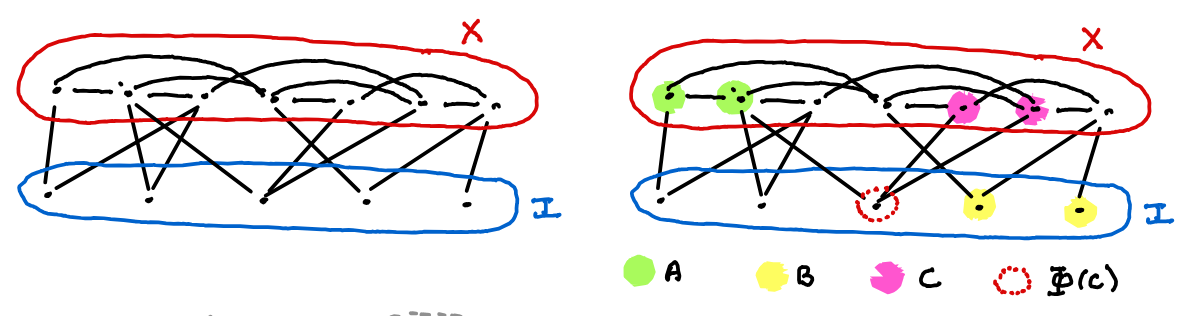
\includegraphics[width=\textwidth]{figures/domset-vc.png}
    \caption{Example of a vertex cover $X$ alongside its independent set $I$. On the right, this illustrates the construction of a dominating set of minimum size $\D = A \uplus B \uplus \Phi(C)$ for a given $A$ (used in the proof of \reftheorem{theorem:domset-vc}).}
    \label{fig:domset-vc}
\end{figure}